% TEMPLATE for Usenix papers, specifically to meet requirements of
%  USENIX '05
% originally a template for producing IEEE-format articles using LaTeX.
%   written by Matthew Ward, CS Department, Worcester Polytechnic Institute.
% adapted by David Beazley for his excellent SWIG paper in Proceedings,
%   Tcl 96
% turned into a smartass generic template by De Clarke, with thanks to
%   both the above pioneers
% use at your own risk.  Complaints to /dev/null.
% make it two column with no page numbering, default is 10 point

% Munged by Fred Douglis <douglis@research.att.com> 10/97 to separate
% the .sty file from the LaTeX source template, so that people can
% more easily include the .sty file into an existing document.  Also
% changed to more closely follow the style guidelines as represented
% by the Word sample file. 

% Note that since 2010, USENIX does not require endnotes. If you want
% foot of page notes, don't include the endnotes package in the 
% usepackage command, below.

% This version uses the latex2e styles, not the very ancient 2.09 stuff.
\documentclass[letterpaper,twocolumn,10pt]{article}
\usepackage{usenix,epsfig,endnotes,enumitem}
\begin{document}

%don't want date printed
\date{}

%make title bold and 14 pt font (Latex default is non-bold, 16 pt)
\title{\Large \bf A Movie Night with Machine Learning}

%for single author (just remove % characters)
\author{
{\rm Michail G.\ Pachilakis}\\
csd3077@csd.uoc.gr
\and
{\rm Iordanis P. Xanthopoulos}\\
csd3161@csd.uoc.gr
% copy the following lines to add more authors
% \and
% {\rm Name}\\
%Name Institution
} % end author

\maketitle

% Use the following at camera-ready time to suppress page numbers.
% Comment it out when you first submit the paper for review.
\thispagestyle{empty}


\subsection*{Abstract}
As the number of movies released continuously grows, viewers are flooded with information about several movie productions, making the simplest questions like "What movie to see tonight?" really hard to answer. Also movie production studios would like to know if a movie could be a commercial success in order to invest money in it.\par In this work \textbf{i.} we provide a simple question interface so the users can find movies matching on his/her creteria, \textbf{ii.} we provide an interface to answer statistic related questions about any movie dataset and \textbf{iii.} we provide predictions about a movies imdb score based on Machine Learning.\\
\\
\textbf{Keywords} Machine Learning; imdb; prediction; spark; statistics; recommendations


\section{Introduction}

A paragraph of text goes here.  Lots of text.  Plenty of interesting
.test.text. \\ 

More fascinating text. Features\endnote{Remember to use endnotes, not footnotes!} galore, plethora of promises.\\

\section{Dataset}

Some embedded literal typset code might 
look like the following :

{\tt \small
\begin{verbatim}
int wrap_fact(ClientData clientData,
              Tcl_Interp *interp,
              int argc, char *argv[]) {
    int result;
    int arg0;
    if (argc != 2) {
        interp->result = "wrong # args";
        return TCL_ERROR;
    }
    arg0 = atoi(argv[1]);
    result = fact(arg0);
    sprintf(interp->result,"%d",result);
    return TCL_OK;
}
\end{verbatim}
}

Now we're going to cite somebody.  Watch for the cite tag.
Here it comes~\cite{Chaum1981,Diffie1976}.  The tilde character (\~{})
in the source means a non-breaking space.  This way, your reference will
always be attached to the word that preceded it, instead of going to the
next line.

\section{Implementation}
We select to implement three different functionalities. The first one targets mostly the movie production studios and is about movie score predictions. The other two are statistics about the movies contained in the dataset and movie recommendations and they mostly target the simple viewers. \par 
For our implementation we used apache spark and the scala programming language. In the subsection 3.1 is described how we implement the movie predictions and in the subsetion 3.2 are described the implementation of movies statistics and the recommendations.
\subsection{Machine Learning}
We implementated the movie score prediction using Machine Learning for this reason we select to use apache spark and scala. Spark provided us with MLlib a scalable machine learning library consisting common learning algorithms and utilities. Also it provides us with spark.ml which aims to provide a uniform set of high-level APIs that help users to create and tune a practical machine learning pipelines. \par 

Firstly we created a case class containg 28 fields, as many as the dataset features, and after parsing the initial dataset we set every feature to it's coresponding class field. We removed from the dataset movies containing commas in their titles because during splitting they generated more features than they should and they generated errors on our comma seperated csv file.\par 

From our initial 28 features we select to keep only those who had meaning for our predictions, so features like "Title", "IMDBLink", "Country" etc. were dropped. We dropped in total 11 features that we thought it would had the least affect in the movie score prediction. \par 

Because our dataset contained a mix of string, double and integer features we had to transform our string features to numeric values. The package spark.ml provides us with the StringIndexer function. StringIndexer converts String values into categorical indices which could me used by machine learning algorithms in ml library.\par 

From our remaing 17 features we had to select only those that would positevly affect prediction of the movie imdb score. To achieve this we correlated our remaining features and excluded those which negatively affected the "imdb\_score" feature. Again the MLlib package provided us with the Statistics package which contained the necessary functions for the feature correlation.\par 

In order to create our machine learning pipeline we had to create some transformers to produce our output dataframe. We created a VectorSlicer which takes a vector as input column and creates a vector containing only the features that we set from the original vector. We also created a StandardScaler which is used to scale a vector to a vector which values are in similar scale and a VectorAssembler which is a feature transformer that merges multiple columns into a vector column.\par 

We initialize the Linear Regression Classifier estimator and then chain it with the VectorSlicer, StandardScaler and VectorAssembler transformers in the machine learning pipeline. When the pipeline is used to fit training data, the transformers and the estimator will apply to the dataframe with the sequence defined in the pipeline.\par 

\subsection{Statistics and Recommendations}

For the Statistics and Recommendations we used map and reduce functions. We used the same case class we described in the section 3.1 to create a RDD with 28 features named \textbf{parsedPointsRdd}. Then we applied filter and ordering functions on it to produce the recommendations. For the statistics we applied filter functions to the \textbf{parsedPointsRdd} and then calculated the statistics. \par 

For statistics we defined the following functions:
\noindent
{\bf \tt GreatMoviesStatistics\((\)):Double } \\ 

\noindent
{\bf \tt DirectorStatistics\((director:String\)):Double } \\ 

\noindent
{\bf \tt GerneStatistics\((gerne:String\)):Double } \\ 

The \textbf{GreatMoviesStatistics} calculates the percentage of the movies that have IMDB score above 8, these are movies that considered top and everyone should probable see them. The \textbf{DirectorStatistics} calculates the percentage of movies that a specific director have directed. The \textbf{GerneStatistics} calculates the percentage of movies included in a specific gerne. \par


For recommendations we defined the following functions:

\noindent
{\bf \tt BestMoviesInCategory\((category:String\)) } \\

\noindent
{\bf \tt findTopTen  \((category:String,language:String,actor1name:String\)) } \\

\noindent
{\bf \tt findTitle\((category:String, language:String, actor1name:String, directorname:String\)) } \\

The \textbf{BestMoviesInCategory} prints the top ten movies in a gerne, specified by the user. The \textbf{findTopTen} prints the top 10 movies based on the gerne, the movie language and the main actors name, these arguments are user specified. Finally the \textbf{findTitle} prints the titles of the movies that match some user specified creteria. The user can specify the gerne of the movie, the language of the movie, the main actors name and the directors name. If some of that arguments are not known  by the viewer it can be left empty by just passing as argument the empty string "". More than one movies can fit the above creteria so we limit the function to return the first ten movie titles based on their imdb score ordering. \par

\bigskip

\begin{figure}
	
	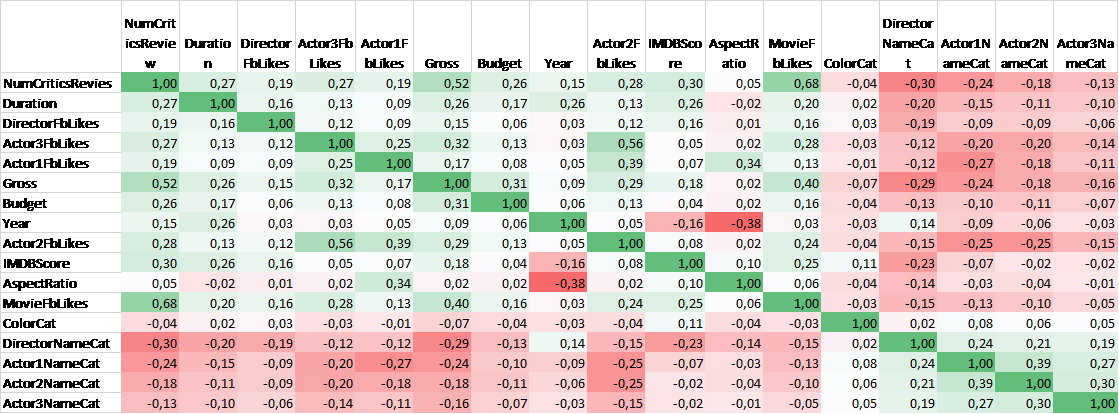
\includegraphics[width=75mm,scale=0.3]{correlation_matrix_image}
	\caption{heatmap of the correlation matrix}
\end{figure}

\section{Results}
In this section we present our machine learning results and evaluate our methodology. We describe in more depth the the correlation process and discuss our evalutation.\par
After loading our dataset and created our dataframe contaiining the 28 movie features we drop the features that we though it will have the least impact with the imdb score feature. These features was: \texttt{"Gerne"}, \texttt{"Title"}, \texttt{"NumVotedUsers"}, \texttt{"CastTotalFbLikes"}, \texttt{"FacesOnPoster"}, \texttt{"PlotKeywords"}, \texttt{"IMDBLink"}, \texttt{"NumUserReviews"}, \texttt{"Language"}, \texttt{"Country"} and \texttt{"ContentRating"}. From these features some can not been created before the movies release sush as \texttt{"NumVotedUsers"} and others can not affect the movie score sush as \texttt{"IMDBLink"}.\par 

We also need to transform the dataframe to convert the String features into numeric features. Then we procced to the correlation which is done using the \texttt{"pearson"} method. In figure 1 we present the heatmap extracted by the features correlation. The more green a cell is the more possitive it correlates with the feature in that row, and the more red a cell is the more negative weight gives in the correlation. Looking at the \texttt{"IMDBScore"} row of the matrix we found that features as \texttt{"Year"}, \texttt{"Actor2Name"}, \texttt{"DirecotrName"}, \texttt{"Actor1Name"} and \texttt{"Actor3Name"} have a negative weight in the imdb score so we drop them.

Using \texttt{randomSplit} we split our dataframe to two datasets. A train dataset containing 80\% of the movies in our initial dataset and a test dataset containing the remaing 20\%. We produce our pipeline model by fitting the training data to our pipeline. The testing data will go though our model to produce the prediction results.\par 

To evaluate our data we created a val \texttt{RegressionEvaluator} which we feed with our previous predictions. The room mean square error we had was 1.02 which considering our features and that the rating scale is from 0 to 10 is acceptable.

We also tested another set of features to make predictions. Based on the Chuan Sun work on the movie predictions we used another set of features. This set includes the following features: "IMDBScore", "DirectorFbLikes", "Duration", "Actor1FbLikes", "Actor2FbLikes", "Actor3FbLikes", "FaceNumOnPostes", "Year", "Color", "Budget". Using our model, because we do not know exactly the parameters used in his model, we had root mean square error 1.04 using these features.  
\section{Conclusion}

A polite author always includes acknowledgments.  Thank everyone,
especially those who funded the work. 

\section{Availability}

You can download the code we used for the machine learning predictions, recommendations and statistics from

\begin{center}
{\tt https://github.com/mipach/imdb/tree/master/src}\\
\end{center}

You can run our code with little or no modications at all, using apache spark. This code is under no license so you can use it free but remeber to refer our work.


{\footnotesize \bibliographystyle{acm}
\bibliography{../common/bibliography}}
lalalalala




\end{document}